\documentclass[a4paper,11pt,openright]{report}
\setlength{\parindent}{0pt} % set noindent for entire file

\usepackage[utf8]{inputenc}
\usepackage[a4paper,top=20mm,bottom=25mm,left=10mm,right=10mm]{geometry}
\usepackage{xcolor,graphicx}
\usepackage{amsmath}
\usepackage{setspace}
\usepackage{sectsty}
\usepackage{etoolbox}
\usepackage{enumitem}
\usepackage{listings}
\usepackage{textcmds}
\usepackage{times}

\graphicspath{ {/home/saran/Analytics/May_05/} }

\lstdefinestyle{mystyle}{
	backgroundcolor=\color{white},
	basicstyle=\ttfamily\footnotesize,
	breakatwhitespace=false,
	breaklines=true,
	captionpos=b,
	keepspaces=true,
	showspaces=false,
	showstringspaces=false,
	showtabs=false,
	tabsize=4
}

\lstset{style=mystyle}

\begin{document}
\singlespacing
\pagestyle{plain}

\begin{center}
\textbf{Assignment t-test} \\
Date: 05/05/2020 \hspace{2mm} Name: D.Saravanan
\end{center}

\vspace{10px}

t-test test the null hypothesis $H_{0}$ against the alternative hypothesis $H_{1}$. \\

For univariate samples, t-test performs a Student $t$ test. The test statistic is assumed to
follow a Student t-Distribution $[df]$. \\ 

For multivariate samples, t-test performs Hotelling's $t^{2}$ test. The test statistic is
assumed to follow a Hotelling t-square distribution $[p,df]$ where $p$ is the dimension of
data. \\

The degrees of freedom $df$, used to specify the distribution of the test statistic, depend 
on the sample size, number of samples, and in the case of two univariate samples, the 
results of a test for equal variances. \\ 

For the t-test, a cutoff $\alpha$ is chosen such that $H_{0}$ is rejected only if $p < 
\alpha$. The value of $\alpha$ used for the \qq{Test Conclusion} and \qq{Short Test 
Conclusion} properties is controlled by the Significance Level option. This value $\alpha$ 
is also used in diagnostic tests of assumptions, including tests for normality, equal 
variance, and symmetry. By default, $\alpha$ is set to $0.05$. \\

\vspace{1cm}

\begin{enumerate}

\item[1.] Two sets of ten students selected at random from a college were taken. One set was
given memory test as they were and the other was given the memory test after two weeks of
training and the scores are given below. \\
\begin{tabular}{lrrrrrrrrrr}
Set A: & 10 & 8 & 7 & 9 & 8 & 10 & 9 & 6 & 7 & 8 \\ 
Set B: & 12 & 8 & 8 & 10 & 8 & 11 & 9 & 8 & 9 & 9 \\
\end{tabular} \\
Do you think there is a significant effect due to training? \\

\textbf{Solution:}

\textbf{Null hypothesis:} $H_{0}: \mu_{1} = \mu_{2}$, \hspace{2px} No significant effect
due to training \\
\textbf{Alternative hypothesis:} $H_{1}: \mu_{1} \neq \mu_{2}$, \hspace{2px} Significant
effect due to training \\

\textbf{Set A:} \\ 
\hspace*{10mm} Mean:
\begin{equation*}
\bar x_{1} = \frac{\sum\limits_{i=1}^{n1} x_{1i}}{n1}
    	= \frac{10 + 8 + 7 + 9 + 8 + 10 + 9 + 6 + 7 + 8}{10}
    	= 8.2
\end{equation*}

\hspace*{10mm} Variance:
\begin{equation*}
s_{1}^{2} = \frac{\sum\limits_{i=1}^{n1} (x_{1i} - \bar {x_{1}})^{2}}{n1 - 1}
		= \frac{\sum\limits_{i=1}^{10} (x_{1i} - 8.2)^{2}}{10 -1} = 1.73333
\end{equation*}

\hspace*{10mm} Standard Deviation:
\begin{equation*}
s_{1} = \sqrt{\frac{\sum\limits_{i=1}^{n1} (x_{1i} - \bar {x_{1}})^{2}}{n1 - 1}}
	= \sqrt{\frac{\sum\limits_{i=1}^{10} (x_{1i} - 8.2)^{2}}{10 -1}}
	= \sqrt{1.73333} = 1.31656
\end{equation*}

\textbf{Set B:} \\
\hspace*{10mm} Mean:
\begin{equation*}
\bar x_{2} = \frac{\sum\limits_{i=1}^{n2} x_{2i}}{n2}
	= \frac{12 + 8 + 8 + 10 + 8 + 11 + 9 + 8 + 9 + 9}{10}
	= 9.2
\end{equation*}

\hspace*{10mm} Variance:
\begin{equation*}
s_{2}^{2} = \frac{\sum\limits_{i=1}^{n2} (x_{2i} - \bar {x_{2}})^{2}}{n2 - 1}
= \frac{\sum\limits_{i=1}^{10} (x_{2i} - 9.2)^{2}}{10 -1} = 1.95556
\end{equation*}

\hspace*{10mm} Standard Deviation:
\begin{equation*}
s_{2} = \sqrt{\frac{\sum\limits_{i=1}^{n2} (x_{2i} - \bar x_{2})^{2}}{n2 - 1}}
= \sqrt{\frac{\sum\limits_{i=1}^{10} (x_{2i} - 9.2)^{2}}{10 -1}}
= \sqrt{1.95556} = 1.39841
\end{equation*} \\

Calculation of $s1/s2$:
\begin{equation*}
\frac{s_{1}}{s_{2}} = \frac{1.31656}{1.39841} = 0.94147
\end{equation*}

Test statistic: 
\begin{equation*}
t = \frac{\bar x_{1} - \bar x_{2}}{\sqrt{s_{1}^{2}/n1 + s_{2}^{2}/n2}}
\end{equation*}

where $n1$ and $n2$ are the sample sizes, $\bar x_{1}$ and $\bar x_{2}$ are the sample
means, and $s_{1}^{2}$ and $s_{2}^{2}$ are the sample variances. 

If equal variances are assumed $(0.5 < s1/s2 < 2)$, then the formula reduces to:
\begin{equation*}
t = \frac{\bar x_{1} - \bar x_{2}}{s_{p} \sqrt{1/n1 + 1/n2}}
\end{equation*}

where
\begin{equation*}
s_{p}^{2} = \frac{(n1-1)s_{1}^{2} + (n2-1)s_{2}^{2}}{n1+n2-2}
\end{equation*}

Calculation of $s_{p}$:
\begin{equation*}
s_{p} = \sqrt{\frac{(10-1) \times 1.31656^{2} + (10-1) \times 1.39841^{2}}{10+10-2}} 
      = 1.35810
\end{equation*}

t-statistic:
\begin{equation*}
t = \frac{8.2 - 9.2}{1.35810 \times \sqrt{1/10 + 1/10}} = -1.64646
\end{equation*}

degrees of freedom:
\begin{equation*}
d.o.f = n_{1} + n_{2} - 2 = 10 + 10 - 2 = 18
\end{equation*}

The critical value for $t$ (from $t$-distribution table) with degrees of freedom $= 18$ and 
$\alpha = 0.05$ is $2.101$ \\

Standard Error:
\begin{equation*}
S.E = s_{p} \sqrt{1/n1 + 1/n2} = 1.35810 \times \sqrt{1/10 + 1/10} = 0.60736
\end{equation*} \\

\textbf{Conclusion:} $|t| < t_{0.05}$, we fail to reject the Null hypothesis. That is there
is no significant effect in the scores of the memeory test due to training.

\pagebreak

Program:
\lstinputlisting[language=Python]{tscript3.py}

\vspace{1cm}

Output:
\lstinputlisting{toutput31.txt}

%figure_1
\begin{figure}[ht!]
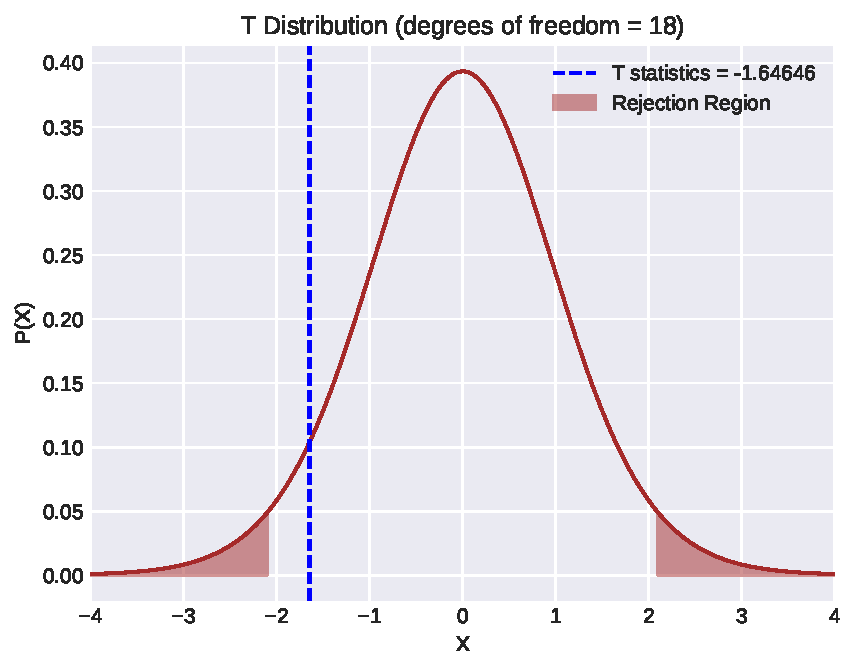
\includegraphics[width=16cm,height=8cm,keepaspectratio]{tscript3.pdf}
\centering
\end{figure}

\vspace{2cm}

Program: t-test with in-built scipy.stats.ttest
\lstinputlisting[language=Python]{ttest2.py}

\vspace{1cm}

Output:
\lstinputlisting{toutput32.txt}

%figure_2
\begin{figure}[ht!]
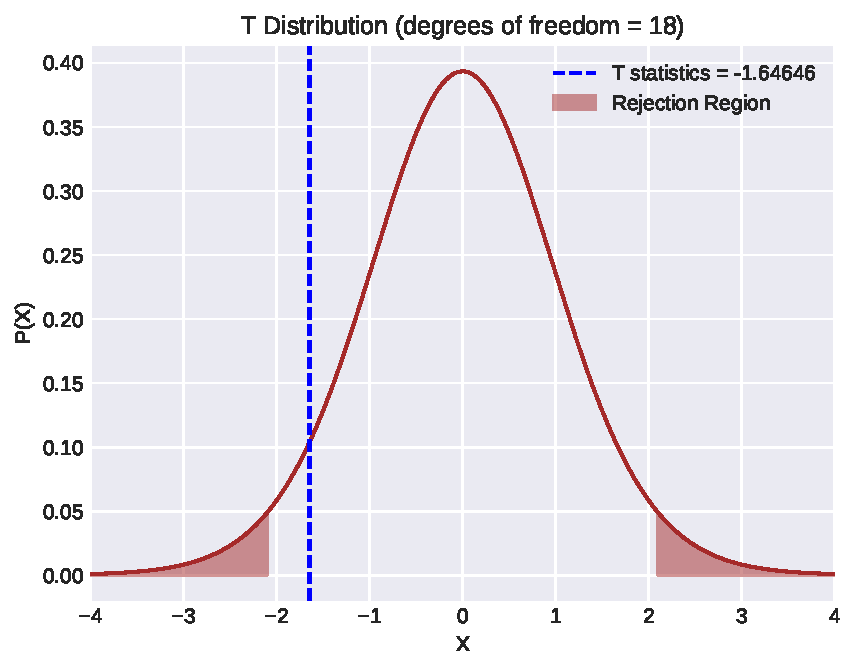
\includegraphics[width=16cm,height=8cm,keepaspectratio]{ttest2.pdf}
\centering
\end{figure}

\vspace{1cm}

\item[2.] A group of 5 patients treated with medicine A weighs 42, 29, 48, 60 and 41 kg.
A second group of 7 patients from the same hospital treated with medicine B weighs 38, 42,
56, 64, 68, 69 and 62 kg. Do you agree with the claim that medicine B increases weight
significantly. \\

\textbf{Solution:}

\textbf{Null hypothesis:} $H_{0}: \mu 1 = \mu 2$, \hspace{2px} No significant increase in
weight \\
\textbf{Alternative hypothesis:} $H_{1}: \mu 1 \neq \mu 2$, \hspace{2px} Significant
increase in weight \\

\textbf{Medicine A:} \\
\hspace*{10mm} Mean:
\begin{equation*}
\bar x_{1} = \frac{\sum\limits_{i=1}^{n1} x_{1i}}{n1}
		= \frac{42 + 29 + 48 + 60 + 41}{5} = 44.0
\end{equation*}

\hspace*{10mm} Variance:
\begin{equation*}
s_{1}^{2} = \frac{\sum\limits_{i=1}^{n1} (x_{1i} - \bar {x_{1}})^{2}}{n1 - 1}
	= \frac{\sum\limits_{i=1}^{5} (x_{1i} - 44.0)^{2}}{5 - 1} = 127.5
\end{equation*}

\hspace*{10mm} Standard Deviation:
\begin{equation*}
s_{1} = \sqrt{\frac{\sum\limits_{i=1}^{n1} (x_{1i} - \bar {x_{1}})^{2}}{n1 - 1}}
	= \sqrt{\frac{\sum\limits_{i=1}^{5} (x_{1i} - 44.0)^{2}}{5 -1}}
	= \sqrt{127.5} = 11.29159
\end{equation*}

\vspace{1cm}

\textbf{Medicine B:} \\
\hspace*{10mm} Mean:
\begin{equation*}
\bar x_{1} = \frac{\sum\limits_{i=1}^{n1} x_{1i}}{n1}
		= \frac{38 + 42 + 56 + 64 + 68 + 69 + 62}{7} = 57.0
\end{equation*}

\hspace*{10mm} Variance:
\begin{equation*}
s_{1}^{2} = \frac{\sum\limits_{i=1}^{n1} (x_{1i} - \bar {x_{1}})^{2}}{n1 - 1}
	= \frac{\sum\limits_{i=1}^{7} (x_{1i} - 57.0)^{2}}{7 - 1} = 154.3
\end{equation*}

\hspace*{10mm} Standard Deviation:
\begin{equation*}
s_{1} = \sqrt{\frac{\sum\limits_{i=1}^{n1} (x_{1i} - \bar {x_{1}})^{2}}{n1 - 1}}
	= \sqrt{\frac{\sum\limits_{i=1}^{7} (x_{1i} - 57.0)^{2}}{7 -1}}
	= \sqrt{154.3} = 12.42310
\end{equation*}

Calculation of $s1/s2$:
\begin{equation*}
\frac{s_{1}}{s_{2}} = \frac{11.29159}{12.42310} = 0.90892
\end{equation*}

Test statistic:
\begin{equation*}
t = \frac{\bar x_{1} - \bar x_{2}}{\sqrt{s_{1}^{2}/n1 + s_{2}^{2}/n2}}
\end{equation*}

If equal variances are assumed $(0.5 < s1/s2 < 2)$, then the formula reduces to:
\begin{equation*}
t = \frac{\bar x_{1} - \bar x_{2}}{s_{p} \sqrt{1/n1 + 1/n2}}
\end{equation*}

where
\begin{equation*}
s_{p}^{2} = \frac{(n1-1)s_{1}^{2} + (n2-1)s_{2}^{2}}{n1+n2-2}
\end{equation*}

Calculation of $s_{p}$:
\begin{equation*}
s_{p} = \sqrt{\frac{(5-1) \times 11.29159^{2} + (7-1) \times 12.42310^{2}}{5+7-2}} 
      = 11.98332
\end{equation*}

t-statistic:
\begin{equation*}
t = \frac{44.0 - 57.0}{11.98332 \times \sqrt{1/5 + 1/7}} = -1.85272
\end{equation*}

degrees of freedom:
\begin{equation*}
d.o.f = n_{1} + n_{2} -2 = 5 + 7 - 2 = 10
\end{equation*}

The critical value for $t$ (from $t$-distribution table) with degrees of freedom $= 10$ and
$\alpha = 0.05$ is $2.228$ \\

Standard Error:
\begin{equation*}
S.E = s_{p} \sqrt{1/n1 + 1/n2} = 11.98332 \times \sqrt{1/5 + 1/7} = 7.01671
\end{equation*}

\textbf{Conclusion:} $|t| < t_{0.05}$, we fail to reject the Null hypothesis. That is there is
no significant increase in weight due to medicine B when compared with medicine A.

\pagebreak

Program:
\lstinputlisting[language=Python]{tscript32.py}

\vspace{1cm}

Output:
\lstinputlisting{toutput41.txt}

%figure_3
\begin{figure}[ht!]
\includegraphics[width=16cm,height=8cm,keepaspectratio]{tscript41.pdf}
\centering
\end{figure}

\pagebreak

Program: t-test with in-built scipy.stats.ttest
\lstinputlisting[language=Python]{ttest22.py}

\vspace{0.5cm}

Output:
\lstinputlisting{toutput42.txt}

%figure_4
\begin{figure}[ht!]
\includegraphics[width=16cm,height=8cm,keepaspectratio]{tscript42.pdf}
\centering
\end{figure}

\vspace{1cm}

\item[3.] Samples of two types of electric bulbs were tested for length of life and the
following data were obtained \\
\begin{tabular}{lrr}
		& Type I & Type II \\
No. of Samples: & 8 & 7 \\
Mean (hours):   & 1134 & 1024 \\
SD (hours):     & 35 & 40 \\
\end{tabular} \\
Test at 5 percent level, whether the difference in sample mean is significant. \\

\textbf{Solution:}

\textbf{Null hypothesis:} $H_{0}: \mu 1 = \mu 2$, \hspace{2px} No significant difference in
sample mean \\
\textbf{Alternative hypothesis:} $H_{1}: \mu 1 \neq \mu 2$, \hspace{2px} Significant
difference in sample mean \\

\textbf{Type I:} \\
\hspace*{10mm} Mean = 1134 \\
\hspace*{10mm} Variance = 1225 \\
\hspace*{10mm} Standard Deviation = 35 \\

\textbf{Type II:} \\
\hspace*{10mm} Mean = 1024 \\
\hspace*{10mm} Variance = 1600 \\
\hspace*{10mm} Standard Deviation = 40 \\

Calculation of $s1/s2$:
\begin{equation*}
\frac{s_{1}}{s_{2}} = \frac{35}{40} = 0.875
\end{equation*}

Test statistic: 
\begin{equation*}
t = \frac{\bar x_{1} - \bar x_{2}}{\sqrt{s_{1}^{2}/n1 + s_{2}^{2}/n2}}
\end{equation*}

where $n1$ and $n2$ are the sample sizes, $\bar x_{1}$ and $\bar x_{2}$ are the sample
means, and $s_{1}^{2}$ and $s_{2}^{2}$ are the sample variances. 

If equal variances are assumed $(0.5 < s1/s2 < 2)$, then the formula reduces to:
\begin{equation*}
t = \frac{\bar x_{1} - \bar x_{2}}{s_{p} \sqrt{1/n1 + 1/n2}}
\end{equation*}

where
\begin{equation*}
s_{p}^{2} = \frac{(n1-1)s_{1}^{2} + (n2-1)s_{2}^{2}}{n1+n2-2}
\end{equation*}

Calculation of $s_{p}$:
\begin{equation*}
s_{p} = \sqrt{\frac{(8-1) \times 35^{2} + (7-1) \times 40^{2}}{8+7-2}} 
      = 37.39087
\end{equation*}

t-statistic:
\begin{equation*}
t = \frac{1134 - 1024}{37.39087 \times \sqrt{1/8 + 1/7}} = 5.68428
\end{equation*}

degrees of freedom:
\begin{equation*}
d.o.f = n_{1} + n_{2} - 2 = 8 + 7 - 2 = 13
\end{equation*}

The critical value for $t$ (from $t$-distribution table) with degrees of freedom $= 13$ and 
$\alpha = 0.05$ is $2.160$ \\

Standard Error:
\begin{equation*}
S.E = s_{p} \sqrt{1/n1 + 1/n2} = 37.39087 \times \sqrt{1/8 + 1/7} = 19.35161
\end{equation*}

\textbf{Conclusion:} $|t| > t_{0.05}$, we reject the Null hypothesis. That is there is 
significant difference in sample mean.

\vspace{2cm}

Program:
\lstinputlisting[language=Python]{t2script3.py}

\vspace{1cm}

Output:
\lstinputlisting{toutput51.txt}

%figure_5
\begin{figure}[ht!]
\includegraphics[width=16cm,height=8cm,keepaspectratio]{t2script3.pdf}
\centering
\end{figure}


%Program: t-test with in-built scipy.stats.ttest
%\lstinputlisting[language=Python]{ttest23.py}
%
%\vspace{1.5cm}
%
%Output:
%\lstinputlisting{t2output3.txt}
%
%\vspace{0.2cm}
%
%%figure_6
%\begin{figure}[ht!]
%\includegraphics[width=16cm,height=8cm,keepaspectratio]{t2script3.pdf}
%\centering
%\end{figure}

\end{enumerate}
\end{document}
